% https://arxiv.org/pdf/2006.05635.pdf
\section{Introduction}

\begin{figure*}[t]
  \centering
  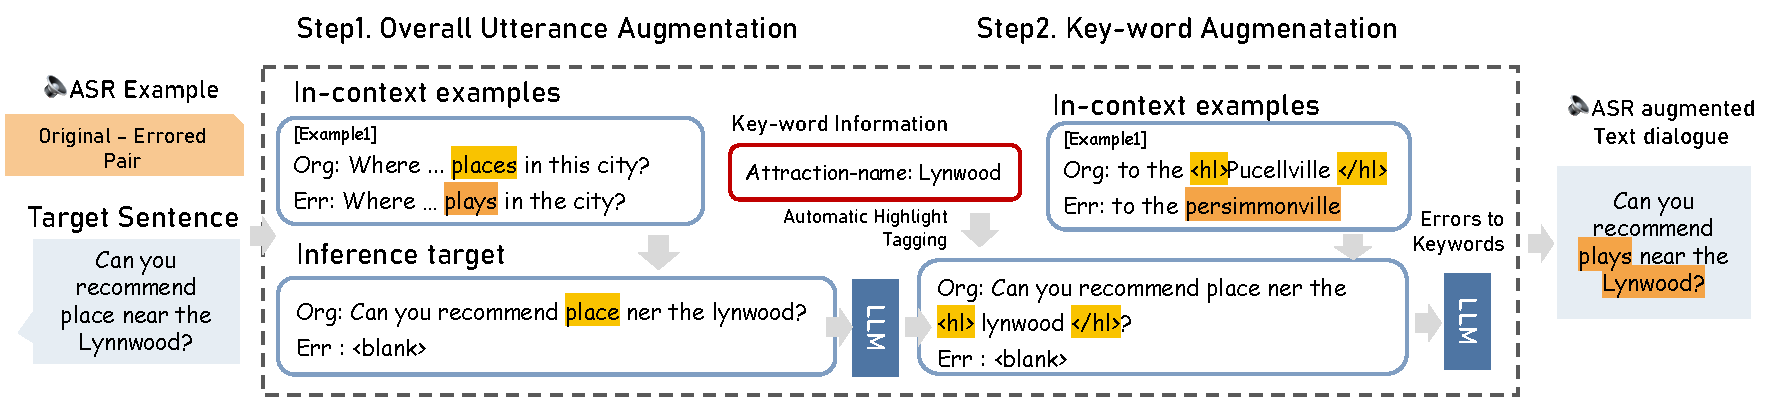
\includegraphics[width=\textwidth]{img/main_image.pdf}
\caption{
Illustration of the EPA process. 
Step~1 introduces overall ASR-like distortions using in-context examples of original–errored pairs, while Step~2 applies keyword-specific phonetic corruptions guided by highlighted slot spans. 
Combining both steps generates realistic and diverse ASR-style errors for robust DST training.
}
   \label{fig:method}
   \vspace{-13pt}
\end{figure*}



Task-oriented dialogue systems (TODs) assist users in achieving specific objectives through conversations and are used in various sectors, including customer service and hotel reservations. A crucial component of these systems is Dialogue State Tracking (DST), which extracts vital information from conversations in a slot-value format (e.g., hotel-name: Claire Hotel). This information is essential for querying databases and generating responses \cite{young2013pomdp}.

However, DST models face significant challenges in spoken dialogue environments, where user utterances are converted into text by automatic speech recognition (ASR) \cite{pal2020modeling, kim2021robust, yoon2023adapting}. Notably, \citet{dstc11} observed a drastic reduction in model accuracy from 41.6\% to 23.6\% in such environments. This decline is primarily due to ASR errors, which frequently misrecognize named entities—a key target in DST \cite{Nechaev2021}.

To address ASR inaccuracies, data augmentation has emerged as a viable, cost-efficient strategy. Existing text augmentation methods, such as word swapping \cite{eda} and back translation \cite{BT}, do not maintain audio similarity with the original text, leading to discrepancies with ASR error patterns. To bridge this gap, \citet{sharma2020improving} and \citet{jacqmin2023olisia} synthesized audio from text with text-to-speech (TTS) model \cite{taco} and processed it through ASR, while \citet{sc-BERT} and \citet{sc-kfold} employed translation model structure to introduce ASR-like errors directly into texts. \citet{huang2020learning} further leveraged word confusion network (WCN) representations for data augmentation to generate acoustically consistent errors. 

Despite these advancements, prior methods often fail to provide sufficient error for DST model training. Accurately identifying key terms is vital for DST performance; thus, models need to be trained on a broad spectrum of ASR-errored keywords. Unfortunately, many current strategies do not ensure that errors are positioned within critical keywords, often generating trivial examples by altering non-essential words such as random words \cite{eda} or sentence structure \cite{BT}. This oversight results in sub-optimal performance against ASR errors.

To address these limitations, we introduce Error Positioning Augmentation (EPA), a straightforward yet effective method that ensures sufficient errors in keywords. Our method leverages large language models (LLMs) \cite{openai, touvron2023llama, zhang2022opt}, which have demonstrated impressive capabilities in semantic augmentation \cite{semaug1, semaug2} and precise text generation control \cite{control1, control2}. Despite their strengths, LLMs' potential for phonetic augmentation remains largely unexplored.

In our method, we utilize in-context learning~\cite{incontext} with phonetically similar examples to introduce general ASR errors and devise a highlighting method to explicitly localize the error to a target span. Surprisingly, without requiring extensive domain-specific user speech data, a publicly available audio dataset and a small set of in-context examples (fewer than 10 samples) are sufficient to generate a wide variety of ASR-errored keywords for DST. This significantly simplifies the error generation process.


In the experiment, to reflect diverse real-world conditions, we evaluated EPA under four ASR environments: a low-accuracy ASR system, noisy audio with café and traffic background, a paraphrased input setting where users naturally rephrased transcriptions, and a high-accuracy ASR system. In these experiments,  EPA significantly improved model robustness, increasing accuracy from 45.76\% to 51.12\% with high keyword diversity (95.4\%), surpassing the previous best-performing model. Our analysis suggests that this improvement is primarily driven by keyword-level augmentation, which effectively mitigates errors in ASR-affected values.

